\section{Řetězec zpracování grafických dat, vektorová a rastrová část a jejich komponenty.}

\textcolor{blue}{Vstupní data \(\rightarrow\) |zpracování vrcholů| \(\rightarrow\) Zpracovaná data vrcholů \(\rightarrow\)} \textcolor{teal}{|rasterizace| \(\rightarrow\) fragmenty (pixely s~hloubkovou pamětí) \(\rightarrow\) |zpracování fragmentů| \(\rightarrow\) |blending| \(\rightarrow\) Barvy pixelů}

Z 3D scény promítá na 2D obrazovku. Skládá se z~\textcolor{blue}{vektorové} a~\textcolor{teal}{rastrové části}.

\subsection{Vstupní data}
\begin{itemize}
    \item Geometrie (souřadnice řídících bodů, jejich normály\dots)
    \item Topologie (kde jsou hrany, plošky a~která strana plošky je viditelná)
    \item Barvy, průhlednost
    \item Charakterizace světel (a~materiálů)
    \item Charakterizace kamery
\end{itemize}

\subsection{Zpracování vrcholů}
\begin{itemize}
    \item Teselace (složitější tvary \(\rightarrow\) jednodušší)
    \item Subdivision (rozdělení, zvětší počet řídících bodů)
    \item Geometrické a~pohledové transformace
    \item Vyhodnocení osvětlení
    \item Projektivní transformace (3D \(\rightarrow\) 2D)
    \item Transformace normál, atributů vrcholů
    \item Souřadnice textur
    \item Ořezání (vše mimo viewing frustum jde pryč)
    \item Vertex Shader
\end{itemize}

\subsection{Zpracovaná data vrcholů}
Primitiva v~obrazovkovém prostoru (jsou 2D)

\subsection{Rasterizace}
Pro každý fragment vypočítána sada hodnot, k~tomu využita interpolace z~vrcholů.
\begin{itemize}
    \item Po trojúhelnících
    \item Rasterizace vnitřních fragmentů trojúhelníku
    \item Interpolace textur
    \item Multisampling nebo jiné potlačení aliasingu
\end{itemize}

\subsection{Fragmenty}
Pixely, ale lepší. Obsahují atributy barvy, průhlednosti\dots

\subsection{Zpracování fragmentů}
\begin{itemize}
    \item Barva a~hloubka pro každý fragment vypočítána.

    \item Postprocessing
\end{itemize}

\subsection{Blending}
\begin{itemize}
    \item Alpha test -- zahodí neviditelné fragmenty
    \item Depth test -- viditelnost podle hloubky (z-buffer)
    \item Alpha blending -- barva podle průhlednosti
\end{itemize}


\section{Světlo. Barva, její měření a její vnímání člověkem. Barevné modely (RGB, CMY, HLS, YCBCR, stupně šedi). Gama korekce.}
Světlo je elmag.\,vlnění mezi 390--720~nm.

Barva je projevem vnímání světla lidským okem. Měří se spektrometrem, avšak lidské oko má pouze tyčinky (jas, desetkrát citlivější) a čípky (R/G/B), různé barvy tedy může vnímat stejně, jelikož je světlo vnímané těmito receptory stejné.

Barva objektu je charakteristikou světla odraženého od objektu, závisí tedy nejen na objektu, ale i~na zdroji světla.

Člověk je nejcitlivější na zelenožluté světlo.

\subsection{Barevné modely}
Abstraktní matematické struktura, popisuje barvu jako n-tici čísel. Není objektivní, pro přesný popis je nutné interpretovat pozorovací podmínky a~další. Pak se z~barevného modelu stane barevný prostor.

\subsection{RGB}
\begin{itemize}
    \item Aditivní model
    \item Podle vnímání barev v lidském oku
    \item Lze vizualizovat jednotkovou krychlí ([0,0,0] je černá, [1,0,0] červená, [1,1,1] bílá atd.)
    \item Vhodný pro monitory
\end{itemize}

\subsection{CMY}
\begin{itemize}
    \item Subtraktivní model
    \item Pigmenty na světlou plochu, vhodný model pro tiskárny
    \item ([0,0,0] je bílá, [1,1,1] je černá)
\end{itemize}

\subsection{HLS}
\begin{itemize}
    \item Hue, Lightness, Saturation
    \item Není krychle, ale kužel
    \item Hue je hlavní spektrální složka
    \item Saturation je sytost, v~podstatě \uv{úzkost} spektra
    \item Lightness (nebo Brightness, Value či Intensity) je jas
    \item Při přechodu po kružnici mezi červenou a fialovou nastane problém nespojitosti vlnové délky
\end{itemize}

\subsection{YCbCr}
\begin{itemize}
    \item Y je luminance
    \item Cb a~Cr jsou chrominance, ve standardu JPEG je daný přesný přepočet na a~z~RGB
    \item Vhodné pro ukládání obrazu, oko je nejvíc citlivé na jas, ten musí být v~největší kvalitě
\end{itemize}

\subsection{Stupně šedi}
\begin{itemize}
    \item Víceméně odpovídá složce Y
    \item Více přístupů, buď aritmetický průměr z RGB nebo vážený průměr
    \item Nejvěrnější výsledek při váženém průměru podle citlivosti oka na danou složku
    \item Např.\,0,6\,G, 0,3\,R, 0,1\,B
\end{itemize}

\subsection{Gama korekce}
\begin{itemize}
    \item Lidské oko nevnímá jas lineárně, ale logaritmicky
    \item Název gama korekce vychází z CRT monitorů, jas odpovídal mocnině vstupního napětí (\(Y=U_{input}^\gamma\))
    \item Prostě jsme více citliví na rozdíly v malé intenzitě. Dvě velké intenzity se od sebe člověku špatně rozpoznávají
    \item Proto je potřeba jas kvantovat neuniformně
    \item Subjektivní jas (L) je závislý logaritmicky na jasu (Y)
\end{itemize}


\section{Obraz jako dvojrozměrný signál. Vzorkování spojitého obrazu, kvantování. Aliasing, moiré.}
Analogový signál je zobrazení \(f:\mathbb{R}^2\rightarrow\mathbb{R}^n\). Každé pozici na obrazovce přiřazují atributy (R, G, B, alpha).

Pokud uvažujeme diskrétní obraz (jen v~pixelech a jen dané hodnoty), je to zobrazení z~diskrétního bodu z~obrazovky o~rozměrech \(x\), \(y\) na diskrétní hodnotu spadající do množiny hodnot \(H_m\): \(f:\{0,1,\dots,N_\mathrm{x}-1\}\times\{0,1,\dots,N_\mathrm{y}\}\rightarrow H_1\times H_2 \times \dots \times H_\mathrm{n}\).

Aby vznikl diskrétní obraz, je nutné spojitý obraz vzorkovat a~kvantovat. Při generování obrazu není úplně nutné vzorkovat a~kvantovat, o~to se starají již části vykreslovacího řetězce.

\subsection{Vzorkování obrazu}
Aby bylo možné vzorkovat bez ztráty informace:

Definice:
\begin{itemize}
    \item Kmitočtově omezený obraz \(f(x,y)\) má \(f_\mathrm{max}<\infty\).
    \item Vzorkovací kmitočet \(f_\mathrm{vz}\) má jednotky spi (sample per inch), ppi (pixel) nebo dpi (dots)
\end{itemize}
Má platit Nyquistovo kritérium, \(f_\mathrm{vz}>2f_\mathrm{max}\)

\begin{itemize}
    \item Při ideálním vzorkování se vzorkuje nekonečně krátký úsek
    \item V reálu se vzorkuje ponějaký úsek, průměr hodnoty zaznamenán
\end{itemize}

\subsection{Kvantování}
= diskretizace spojité škály signálu

\begin{itemize}
    \item Vzniká kvantizační šum
    \item Škála může a nemusí být uniformní. Obzvláště pro jas je vhodné neuniformní kvantování
\end{itemize}

\subsection{Aliasing}
= V rekonstruovaném obrazu se mění kmitočtový rozsah

\begin{itemize}
    \item Nastane, pokud není obrazová funkce kmitočtově omezená nebo není splněno Nyquistovo kritérium
    \item Příliš vysoké frekvence nejsou správně zachyceny a~ovlivňují nižší frekvence
    \item Mohou se změnit fáze obsažených složek
    \item Mohou se objevit nové kmitočty
\end{itemize}

Předcházení:
\begin{itemize}
    \item Antialiasingový filtr: mírné rozmazání
    \item Supersampling (nadvzorkování) (Supersampling posouvá problém k~vyšším frekvencím, aliasing není tak výrazný)
    \item Vzorkování s~prvkem náhody -- naruší uniformnost vzorkování
\end{itemize}

\subsection{Moiré}
Původní obrazce mohou měnit tvar nebo strukturu (nekonečná šachovnice)



\section{Základy vektorové grafiky. Matematický popis 2D křivek, řídicí body. Typy navázání dvou křivek.}
Užívá se vektorů, matic, vektorového a~skalárního součinu a~taky polynomů.

\subsection{Křivky}
Definice:
\begin{itemize}
    \item explicitně: \(y=f(x)\)
    \item implicitně: \(F(x,y)=0\)
    \item parametricky: \(q(t)=[x(t),y(t)]\), \(t\in[t_\mathrm{min},t_\mathrm{max}]\)
\end{itemize}

Také má řídící body, ty křivku přesně určují. Má většinou splňovat:
\begin{itemize}
    \item Křivka leží v~konvexní obálce svých ř.\,bodů
    \item Změna polohy 1 řídícího bodu změní okolí bodu, ne celou křivku
    \item Krajními řídícími body křivka prochází
    \item Invariance vůči lineárním transformacím
\end{itemize}

Užívaný zápis kubiky: \(\mathrm{\textbf{q}}(t)=\begin{bmatrix}
    t^3 & t^2 & t & 1
\end{bmatrix}
\begin{bmatrix}
    a_x & a_y \\
    b_x & b_y \\
    c_x & c_y \\
    d_x & d_y \\
\end{bmatrix}
=\mathrm{\textbf{TC}}\)

Ale není jasné, jaký je vztah matice \textbf{C} a~řídících bodů. Proto se také používá \(\textbf{q}(t)=\textbf{TMG}\), kde \textbf{T} je stejné, ale \textbf{G} jsou souřadnice řídících bodů. \textbf{M} je bázová matice, stejná pro daný typ křivky.

\subsection{Beziérovy křivky}
\(\textbf{q}^\mathrm{Bez}(t)=\sum^n_{k=0}\mathbf{P}_kB_{k,n}(t)\),
P jsou řídící body, je jich n+1. B jsou Bernsteinovy polynomy (\(B_{k,n}=\left(\begin{array}{c}
    n \\
    k
\end{array}\right)t^k(1-t)^{n-k}
\), \(t\in[0,1]\), \(k=0, 1, \dots,n\))


\subsection{Typy navázání dvou křivek}

\begin{itemize}
    \item Parametrické
    \begin{itemize}
        \item \(C^n\)-spojité
        \item \(\mathbf{q}_1^{(k)}(1)=\mathbf{q}_2^{(k)}(0)\) pro \(k=0,1,\dots,n\)
        \item Tzn.\.derivace nultá až \(n\)-tá v~koncovém bodu první křivky je stejná jako derivace stejného řádu v~počátečním bodu druhé křivky 
    \end{itemize}
    \item Geometrické
    \begin{itemize}
        \item \(G^n\)-spojité
        \item \(\mathbf{q}_1^{(k)}(1)=m_k\cdot \mathbf{q}_2^{(k)}(0)\), \(k=0,1\dots,n\), \(m_k>0\)
        \item Tzn.\,derivace nultá až \(n\)-tá v~koncovém bodu první křivky je lineární kombinací derivace stejného řádu v~počátečním bodu druhé křivky
        \item Prostě stejný směr vektorů, ale můžou mít jinou délku
    \end{itemize}
\end{itemize}


\section{Princip a postup rasterizace základních prvků – úsečka, kružnice, elipsa; trojúhelník.}
\subsection{Rasterizace úsečky}
\begin{itemize}
    \item Algoritmus DDA
    \begin{itemize}
        \item Směrnice (\(m\)) z krajních bodů
        \item zvyšuje v~každém kroku \(x\)~o~1, \(y\)~o~směrnici
        \item Zaokrouhlení dolů nebo nahoru
        \item Funguje jen pro \(m\leq1\)
    \end{itemize}
    \item Bresenhamův algoritmus
    \begin{itemize}
        \item Využívá celočíselnou aritmetiku, může zrychlit výpočet
    \end{itemize}
    \item Mid-point alg
    \begin{itemize}
        \item Pracuje s~implicitním tvarem úsečky, jinak vychází z~Bresenhamova
    \end{itemize}
\end{itemize}

\subsection{Rasterizace kružnice}
\begin{itemize}
    \item Využije se jeden z~algoritmů typu DDA (třeba Bresenhamův) pro jednu osminu
    \item Zrcadlení na ostatní kvadranty
\end{itemize}

\subsection{Rasterizace elipsy}
\begin{itemize}
    \item Obdobně jako kružnice, ale symetrické jsou jen kvadranty
    \item Kvadranty musí následovat osy elipsy
    \item Při počítání v explicitním tvaru je nutné taky během výpočtu změnit kartézskou osu, ať je dodržena podmínka \(m\leq1\)
\end{itemize}

\subsection{Rasterizace trojúhelníku}
\begin{itemize}
    \item Nutné barycentrické souřadnice
    \begin{itemize}
        \item vrcholy A,B,C, barycentrické souřadnice \(\alpha, \beta, \gamma\) jsou počítané \(\alpha\mathbf{A}+\beta\mathbf{B}+\gamma\mathbf{C}\), \(\alpha+\beta+\gamma=1\)
    \end{itemize}
    \item Nalezen nejmenší obdélník obsahující trojúhelník
    \item Pixel po pixelu jsou počítané barycentrické souřadnice
    \item Pokud všechny souřadnice jsou větší než 0, spočítá barvu podle souřadnic (vážený průměr)\(\mathbf{c}(x,y)=\alpha\mathbf{c_A}+\beta\mathbf{c_B}-\gamma\mathbf{c_C}\)
\end{itemize}

\section{Pláty a Bézierovy bikubiky v 3D, řídicí body. Typy navazování plátů. Algoritmus de Casteljau pro jejich polygonizaci, subdivision. Homogenní souřadnice a jejich použití při geometrických transformacích (posun, rotace, změna měřítka a podobně).}
\subsection{Pláty}
\(\mathbf{q}(u,v)=\begin{bmatrix}
    x(u,v) & y(u,v) & z(u,v)
\end{bmatrix}\), \(u,v\in[0,1]\) (mají 2 \uv{časové} složky), 3 souřadnice

\subsection{Beziérovy pláty}
\begin{itemize}
    \item Mají 16 řídících bodů.
    \item \(\mathbf{q}^\mathrm{Bez}(u,v)=\sum^n_{i=0}\sum^m_{j=0}\mathbf{P}_{ij}B_{i,n}(u)B_{j,m}(v)\), \(u\in [0,1], v\in [0,1]\)
    \item \(x(u,v)=\mathbf{UMG}_x\mathbf{M}^\mathrm{T}\mathbf{V}^\mathrm{T}=\begin{bmatrix}
        u^3&u^2&u&1
    \end{bmatrix}\mathbf{MG}_x\mathbf{M}^\mathrm{T}\begin{bmatrix}
        v^3 \\ v^2 \\ v \\ 1
    \end{bmatrix}\) a~stejně pro další souřadnice
\end{itemize}

\subsection{Navazování plátů}
Obdobně jako předchozí navazování, minimální nárok je \(C^0\)

\subsection{Alg.\,de Casteljau}
Pro 2D křivku:
\begin{itemize}
    \item Spojím řídící body
    \item Zvolím krok \(\Delta t\)
    \item Posunu se o~krok na každé ze 3 spojnic řídících bodů, umístím tam bod
    \item Spojím body, mám 2 úsečky
    \item Na nich o~stejný krok opět vytvořím body, spojím
    \item Mám úsečku. Na ní taky zvolím bod podle kroku
    \item Mám jeden bod. Inkrementuju krok a opakuju
    \item Spojením bodů získám polynomizovanou křivku
\end{itemize}

Pro 3D plát je to stejné, jen je potřeba to stejné udělat pro \(u\) a~\(v\). Je jedno, který směr začne.

\subsection{Subdivision de Casteljau}
Vychází z~de Casteljau v~bodě \(t=0,5\), nové řídící body jsou odvozeny od pomocných bodů z~výpočtu. V obrázku~\ref{fig:subdivision-decasteljau} budou nové řídící body \(\begin{bmatrix}
    b_0^0 & b_0^1 & b_0^2 & b_0^3
\end{bmatrix}\) a \(\begin{bmatrix}
    b_0^3 & b_1^2 & b_2^1 & b_3^0
\end{bmatrix}\)

\begin{figure}
    \centering
    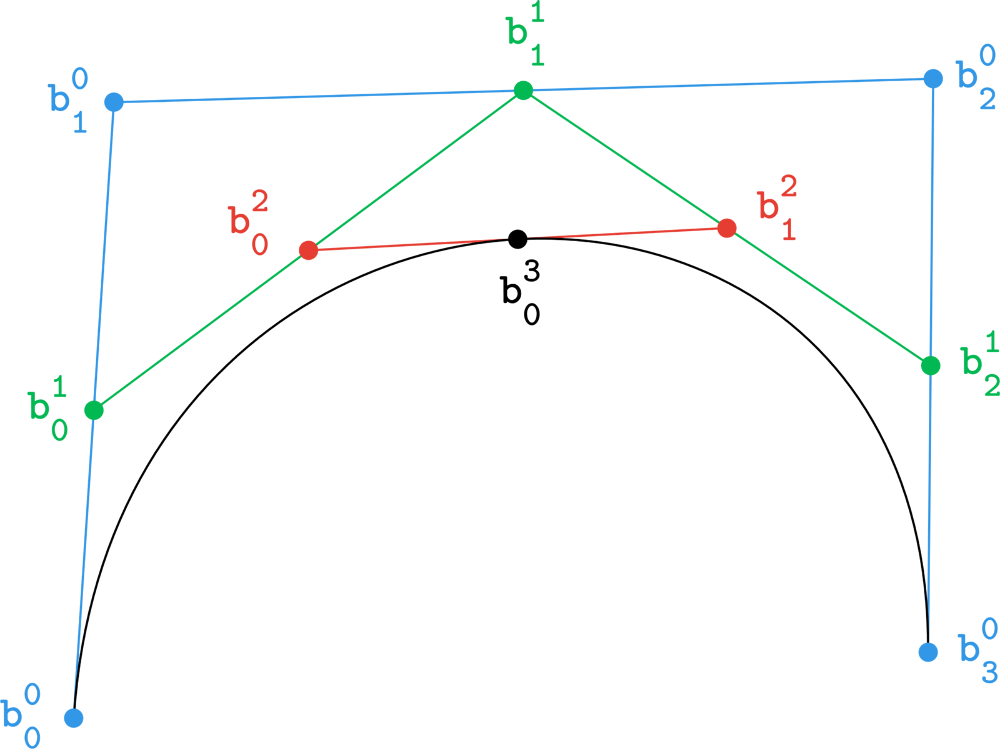
\includegraphics[width=0.8\textwidth]{obrazky/deCasteljau.png}
    \caption{Subdivision pomocí de Casteljau}
    \label{fig:subdivision-decasteljau}
\end{figure}

\subsection{Homogenní souřadnice}
Jedná se o~čtyřrozměrné souřadnice (pro 3D body), kde 4.\,souřadnice udává \uv{váhu}.

Převod z~kartézských: přidat souřadnici o~hodnotě 1.

Převod do kartézských: Každou souřadnici podělit \uv{váhou}.

Umožňují posunutí objektu maticovým násobením. Jeden kartézský bod může mít nekonečně homogenních ekvivalentů. Umožňují také umístit bod do nekonečna (nastaví \uv{váhu} na 0).

\subsection{Geometrické transformace}

Homogenní souřadnice lze lehce využít k~aplikování transformací: \(\mathbf{A}\cdot\mathbf{P}_\mathrm{hom}\)

\subsection{Posun}

\(\mathbf{A}=\begin{bmatrix}
    1 & 0 & 0 & t_x \\
    0 & 1 & 0 & t_y \\
    0 & 0 & 1 & t_z \\
    0 & 0 & 0 & 1
\end{bmatrix}\)

\subsection{Rotace}
Kolem osy \(z\) o úhel \(\alpha\):

\(\mathbf{A}=\begin{bmatrix}
    \cos \alpha & -\sin \alpha &0 & 0 \\
    \sin \alpha & \cos \alpha & 0 & 0 \\
    0 & 0 & 1 & 0 \\
    0 & 0 & 0 & 1 \\
\end{bmatrix}\)

\subsection{Změna  měřítka}
\(\mathbf{A}=\begin{bmatrix}
    s_x & 0 & 0 & 0 \\
    0 & s_y & 0 & 0 \\
    0 & 0 & s_z & 0 \\
    0 & 0 & 0 & 1\\
\end{bmatrix}\)

\section{Promítání rovnoběžné a středové, pohledový objem. Osvětlování, Phongův lokální osvětlovací model, globální zobrazovací metody.}
\subsection{Promítání}
= projekce

\begin{itemize}
    \item Jedná se o~převod z~3D do 2D
    \item Existují 2 souřadnicové systémy:
    \begin{itemize}
        \item WCS = world coordinate system (neměnný)
        \item VCS = viewing coordinate system (podle kamery)
    \end{itemize}
    \item Pro převod z WCS na VCS: \(\mathbf{P}'=\mathbf{T_\mathrm{proj}}\cdot\mathbf{T}_\mathrm{cam}\cdot\mathbf{T}_\mathrm{world}\cdot\mathbf{P}\)
    \item Matice kamery závisí na souřadnicích, směr pohledu a~na vektoru ukazující, co je nahoře
    \item Matice světa je identita, pokud se kamera kouká na výchozí pozici osy z kolmo na průmětnu
\end{itemize}

\subsection{Rovnoběžné promítání}
\begin{itemize}
    \item Promítací paprsky jsou rovnoběžné
    \item \(\mathbf{T_\mathrm{proj}=\begin{bmatrix}
        1 & 0 & 0 & 0 \\
        0 & 1 & 0 & 0 \\
        0 & 0 & 0 & z_0 \\
        0 & 0 & 0 & 1 \\
    \end{bmatrix}}\), pokud je průmětnou rovina \(z=z_0\)
    \item Půdorys/bokorys/nárys
\end{itemize}

\subsection{Středové promítání}
\begin{itemize}
    \item Perspektivní
    \item \(\mathbf{T_\mathrm{proj}=\begin{bmatrix}
        1 & 0 & 0 & 0 \\
        0 & 1 & 0 & 0 \\
        0 & 0 & 0 & 0 \\
        0 & 0 & -1/z_0 & 1 \\
    \end{bmatrix}}\), pokud je průmětnou rovina \(z=z_0\)
\end{itemize}

\subsection{Pohledový objem}
\begin{itemize}
    \item Omezení množství objektů ke zpracování, objekty mimo nejsou zpracovávány
    \item Definováno pomocí \textit{near clipping plane} a~\textit{far clipping plane}
    \item z-buffer je potom číslo závislé na rozdílu těchto planes. Pokud jsou dostatečně blízko, má buffer dostatečné rozlišení
    \item Pokud rozlišení nemá, může dojít ke clipping effectu
\end{itemize}

\subsection{Osvětlování}
Zdroje světla:

\begin{itemize}
    \item bodový
    \item směrový (bodový, ale jen v~kuželu)
    \item plošný
\end{itemize}

Modely:

\begin{itemize}
    \item Lokální -- Každý bod zvlášť, neřeší zastínění či odrazy světla od okolních objektů
    \item Globální -- Ray Tracing (sledování paprsku z~kamery k~objektu, pak do zdroje světla, rekurze\dots)
\end{itemize}

\subsection{Phongův lokální osvětlovací model}

3 složky světla:
\begin{itemize}
    \item Ambientní (i bez zdroje světla)
    \item Difúzní (udává barvu)
    \begin{itemize}
        \item \(L_\mathrm{d}=c_\mathrm{d}\cdot I\cdot\mathrm{max}\{0,\langle \mathbf{n}, \mathbf{l}\rangle \}\), kde \(c_\mathrm{d}\) je difúzní reflektance, \(I\) je nominální intenzita světla a \(\langle\mathbf{n}, \mathbf{l}\rangle\) je skalární součin normály a~vektoru ke zdroji světla
        \item Nezáleží na pozorovateli
    \end{itemize}
    \item Spekulární
    \begin{itemize}
        \item \(L_\mathrm{s}=c_\mathrm{s}\cdot I\cdot(\mathrm{max}\{0,\langle \mathbf{n}, \mathbf{h}\rangle \})^p\), kde \(h=\frac{\mathbf{v}+\mathbf{l}}{||\mathbf{v}+\mathbf{l}||}\), \(v\) je vektor ke kameře a~\(p\) ovlivňuje šířku odrazu
    \end{itemize}
    \item max je tam, aby se nepočítaly tupé úhly, ty by musely vycházet z~tělesa ven, jednalo by se o~zastíněnou stranu
\end{itemize}

\subsection{Globální zobrazovací metody}
= ray tracing

3 kroky:
\begin{itemize}
    \item Vytvoření paprsku z~kamery skrz pixel (fragment) na zobrazovací rovině
    \item Nalezení průsečíku s~objektem
    \item Získání barvy (sledování paprsku dále k~původci světla, musí být rekurzivní)
\end{itemize}

Také umožňují vrhat stíny


\section{Texturování, mapování 2D textur na 3D objekt, interpolace textur, komprese textur. Bitmapové a procedurální textury.}
Textura charakterizuje povrch tělesa

Dělení textur:
\begin{itemize}
    \item barva
    \item množství odraženého světla
    \item průhlednost
    \item zvrásnění
    \item hypertextura (co je nad povrchem --tráva, vlasy\dots)
\end{itemize}

Nebo podle dimenzí:
\begin{itemize}
    \item 1D: přerušovaná čára
    \item 2D: povrch těles
    \item 3D: materiál
    \item 4D: animovaná 3D textura
\end{itemize}

Nebo podle vzniku:
\begin{itemize}
    \item Rastrové
    \item Procedurální
\end{itemize}

\subsection{Mapování 2D textur na 3D objekt}
Texturu popišme texturovací funkcí \(T(u,v)\), funkce inverzního mapování je pak \(M(x,y,z)\), přiřazuje každému bodu z~povrchu tělesa bod z~textury.

Využití pro získání barvy: \(b=T(u,v)=T(M(x,y,z))\)

\subsection{Interpolace textur}
Zvláště u rastrových textur, nemusí vycházet souřadnice na přesný bod, ten je pak potřeba interpolovat. Možnosti:
\begin{itemize}
    \item lineární interpolace (1D data)
    \item bilineární (2D data)
    \item trilineární (3D data)
\end{itemize}
Víceméně jde jen o~počet opakování interpolace.

\subsection{Komprese textur}
\subsubsection{MIP-mapping}
Jedná se spíš o~opak komprese, v paměti se předpočítá textura pro různé velikosti. Interpolace z~větší a~menší textury.

\subsubsection{S3TC}
\begin{itemize}
    \item bloky \(4\times4\)
    \item Nalezení dvou extrémních barev, 16 b (5 pro R, 6 pro G, 5 pro B) pro každou z~nich
    \item Další 2 barvy se interpolují z~těchto extrémů
    \item Každý texel dostane jednu ze 4 barev z~indexové tabulky
    \item Pevný kompresní poměr, 4:1
\end{itemize}

\subsubsection{3DFX Interactive}
Navazuje na S3TC, další 4 módy
\begin{itemize}
    \item CC\_MIXED = S3TC
    \item CC\_HI (\(4\times8 bloky\),  2 barvy, pak dalších 5 intrapolovat, osmá je transparentní, 3b na texel)
    \item CC\_CHROMA (\(4\times8\), 4 barvy po 15 b, bez interpolace, 2b na texel)
    \item CC\_ALPHA (\(4\times8\), 3 barvy po 20 b s průhledností, 2 pro levý a~2 pro pravý blok, nalevém i pravém se interpolují 2 další barvy, 2b na texel
\end{itemize}

Výběr podle střední kvadratické chyby.

\subsection{Bitmapové textury}
Uložené jako rastr (texely).

\subsection{Procedurální textury}
Šumová funkce, využity Perlinovy šumové funkce.

Pro generování textur se užívá více šumů s~různými amplitudami přeloženy přes sebe.

\(h_\mathrm{sum}(x;,p,n)=\sum_{i=0}^{n-1}p^ih(2^ix)\)

Na základě šumu jsou generovány vzory, které se opakují a mají vypadat organicky (mramor, dřevo, mraky). Persistence \(p\) určuje rychlost klesání amplitud vyšších frekvencí. Oktávy jsou pak mocniny 2 udávající frekvence šumu.

\section{Třídění paralelních systémů. Proudové zpracování instrukcí, cache. Paralelní procesory. Technologie SIMD.}
\subsection{Třídění podle Flynna}
\begin{itemize}
    \item SISD -- sériové zpracování
    \item MISD -- multiple instructions stream, single data stream, např.\,databáze
    \item SIMD -- více jednotek zpracovává stejná data
    \item MIMD -- obecný paralelní systém
\end{itemize}

\subsection{Proudové zpracování dat}

\begin{itemize}
    \item Hodinový cyklus: perioda hodinového signálu
    \item Strojový cyklus: časový interval potřebný k~provedení instrukce (třeba 3 hodinové takty, různé pro různé instrukce)
\end{itemize}

Instrukci provádí několik specializovaných jednotek, každá obsluhuje jinou fázi instrukce. Různé fáze jsou prováděny současně na různých jednotkách. Problém je větvení programu. Používá se \textit{predikce větvení}, jsou zahozeny všechny následující instrukce při nesprávně uhádnutém větvení. V~opačném případě dojde k~úspoře.

\subsection{Cache}
Vyrovnávací paměť architektury SRAM (odlišit od DRAM na RAM). Čím menší, tím méně informace pojme, ale tím rychlejší je do ní přístup. Proto jsou 3 úrovně:

\begin{itemize}
    \item L1: na čipu blízko procesoru, malá a~rychlí
    \item L2: na čipu, více místa, menší rychlost
    \item L3: Sdílená mezi více jádry
\end{itemize}

Cache hit: hledaná paměť nalezena. Jinak cahce miss.

Paměť se hledá prvně na L1, pak L2, L3 a~nakonec v~RAM. Počet cyklů potřebných závisí na tom, kde byla paměť nalezena.

Užívají se odlišené cache pro instrukce a~data (Harvardská architektura) nebo sdílená pro oba  typy (Von Neumannova architektura).

\subsection{Paralelní procesory}
\begin{itemize}
    \item Úlohový paralelismus: zpracovává více programů souběžně
    \item Datový paralelismus: SIMD -- data nezávislá na ostatních, uložení dat do registrů za sebou (podle velikosti dat se vejde různé množství, registry mají pevně danou délku)
\end{itemize}

Granularita:
\begin{itemize}
    \item coarse-grained -- menší množství velkých výpočtů, menší režie, nemusí být tak efektivní
    \item fine-grained -- velké množstvý rychlých výpočtů, potřeba více režie, ale možné velké zrychlení
\end{itemize}

Paralelní systémy na jednom čipu:
\begin{itemize}
    \item Čtení a zpracování s~více přístupy (VLIW, VLES, (instrukční packety, instrukce z~nich rozděleny mezi jednotky programátorem) superskalární architektura (všechny moderní CPU, instrukční packety rozděluje plánovač))
    \item Úlohový paralelismus (vícejaderné a~hyper-threading (má více architectural states v~jádře -- více vláken))
    \item Datový paralelismus (SIMD a grafické procesory)
\end{itemize}


\section{Architektury moderních grafických procesorů (GPU). GPU jako paralelní systém pro grafické i obecné výpočty. Vertex shader, pixel shader.}

\subsection{Architektura DirectX9}
Viz obrázek~\ref{fig:architektura-gpu}.
\begin{figure}
    \centering
    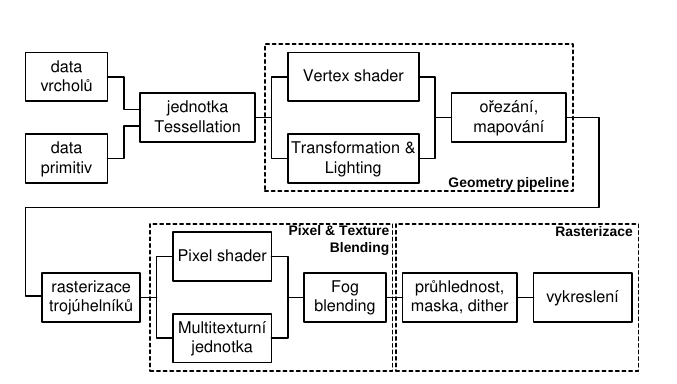
\includegraphics[width=\linewidth]{obrazky/architekturaGPU.png}
    \caption{Architektura DirectX9}
    \label{fig:architektura-gpu}
\end{figure}

\subsection{Architektura paměti GPU}
Viz obrázek~\ref{fig:architektura-pamet}.
\begin{figure}
    \centering
    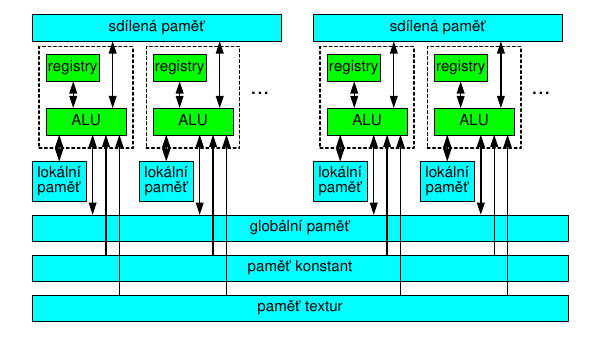
\includegraphics[width=\linewidth]{obrazky/architektura-pamet-gpu.png}
    \caption{Architektura paměti v GPU}
    \label{fig:architektura-pamet}
\end{figure}

Příklad architektury: Nvidia Blackwell (RTX 5090) -- 8 Texture Processing Clusters, každý 2 Streaming multiprocessor, každý z~nich 128 CUDA jader, 1 ray-tracing jádro, 4 tenzorová vlákna, 4 texturovací jednotky, 256 kB registrů, 128 kB L1 cache.

\subsection{GPU jako paralelní systém pro grafické i~obecné výpočty}
Slovník:
\begin{itemize}
    \item Kernel: kód k~vykonání na GPU
    \item Vlákno: programové vlákno, vykonává kernel
    \item Blok: Skupina vláken, sdílí data a~synchronizační bod
    \item Síť: Skupina bloků, sdílí kernel, ale ne data a~synchronizační bod
\end{itemize}

Shader se mění ve vícejádrový procesor, má i lokální a sdílenou cache.

Používá se např.\,CUDA

\subsubsection{CUDA}
1 host (CPU) a zařízení (grafické karty), jazyk vychází z~C a~má části, které jsou pro hosta a~pro zařízení. Pro alokování paměti na kartě je potřeba speciální funkce (\texttt{cudaMalloc}, \texttt{cudaFree}, \texttt{cudaMemcpy}).

Obsahuje identifikátory:
\begin{itemize}
    \item \texttt{blockIdx}
    \item \texttt{threadIdx}
    \item \texttt{blockDim}
\end{itemize}

\subsection{Vertex Shader}
Datové slovo má 128 b, většinou rozdělené na 4 části (X, Y, Z, W -- souřadnice a viewport). Zpracovává data vrcholů v~3D prostoru. Příklad: bump-mapping (aplikace textury nerovnosti) -- do registrů je předána textura, z~ní pak shader vyčte data, upraví normálu a~zapíše do výstupních registrů.

\subsection{Pixel Shader}

Zpracování pixelů po rasterizaci, uživatelsky definované. Jednomu pixelu odpovídá více fragmentů. Podobná architektura jako vertex shader, liší se využití registrů (X--Z jsou RGB, W je alpha).

Programování shaderů je nutné buď v assembly nebo zkompilovat výstup z vyššího jazyka (HLSL = high level shader language).